\chapter{Programación en GPU}
\graphicspath{{figs/cap4/}}
\label{cap4}

\section{Programación CUDA C}

El procesador principal que tiene una PC es la CPU, por lo cual se denomina \textit{host}, la GPU es un coprocesador y se denomina \textit{device}. Las ejecuciones de los procesos en la CPU están diseñadas para que se efectúen de manera secuecnial, en cuánto las de la GPU en paralelo; las últimas realizándose en varios hilos de ejecución (\textit{threads}). Las operaciones en paralelo que son analizadas por la CPU y las refiere a la GPU son llevadas a cabo mediante funciones llamadas \textit{kernel}. \textit{Host} y \textit{device} poseen su propia memoria RAM, llamadas \textit{host memory} y \textit{device memory} respectivamente. \cite{rinaldi2011modelos}

\begin{figure}[h!]
	\centering
	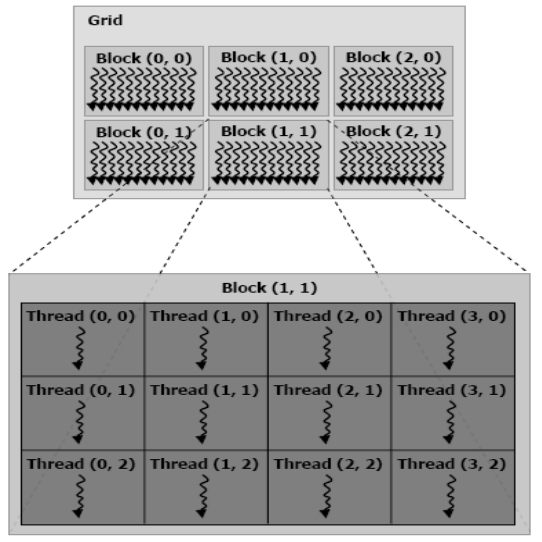
\includegraphics[width=0.4\textwidth]{figs/cap4/threads_block_grid.png}
	\caption{Bloques de threads organizados en una grilla de bloques \cite{rinaldi2011modelos}.}
	\label{fig:block_grid_threads}
\end{figure}

Un bloque de \textit{threads} (\textit{thread block}) es un grupo de hilos de ejecución que pueden cooperar entre sí compartiendo eficientemente datos a través de la memoria compartida de acceso rápido y sincronizando sus ejecuciones, lo cual permite coordinar el acceso a los datos especificando puntos de sincronización en el \textit{kernel}. 

Una grilla de bloques es una agrupación de (\textit{thread block}) que ejecutan el mismo \textit{kernel}. Ésto vence la limitación de hardware que hay un limitado número de \textit{threads} por bloque. Debido a que la ejecución del proceso en los bloques de \textit{threads} de una grilla pueden ser realizados en tiempos distintos, es necesario realizar un sincronización entre los mismos para que su comunicación sea segura y no haya conflictos.\label{prob:sync} \cite{tolke2010implementation}

La figura \ref{fig:block_grid_threads} muestra el concepto de grilla de bloques y (\textit{thread block}).

La programación de las GPU se realiza mediante el lenguaje CUDA, el cuál es una extención del lenguaje C debido su familiaridad y uso extendido, por lo que el lenguaje se denomina CUDA C. La realización de procesos en paralelos es llevada a cabo mediante funciones llamadas \textit{kernel} y son del tipo \textit{void}.

Existen tres tipos de funciones que se pueden llevar a cabo y son:

\begin{itemize}
	
	\item \textbf{host} función clásica de C que se ejecuta en la CPU, siendo invocable únicamente por funciones que se ejecuten en la CPU. 

	\item \textbf{global} es una función \textit{kernel} invocada desde la CPU para ejecutarse en la GPU. 
%	Debe especificar la cantidad de bloques y de \textit{threads} por bloque a lanzar la función.
	
	\item \textbf{device} es una función que se ejecuta en la GPU y únicamente puede ser llamada desde un \textit{kernel}.
	
\end{itemize}

La allocación de memoria en el \textit{host} es la misma que se utiliza en C: \textbf{malloc($\>$)}, mientras que en el \textit{device} se realiza mediante: \textbf{cudaMalloc($\>$)}, la cual recibe los siguientes argumentos:
{\footnotesize
\begin{frame}{}
	\lstset{language=C,
		framesep=2mm,
		basicstyle=\ttfamily,
		keywordstyle=\color{blue}\ttfamily,
		stringstyle=\color{red}\ttfamily,
		commentstyle=\color{green}\ttfamily,
		morecomment=[l][\color{magenta}]{\#}
	}
	\begin{lstlisting}
cudaMalloc(void **devPtr, size_t size);
	\end{lstlisting}

\end{frame}
}
(devPtr) puntero para allocar la memoria del \textit{device} , (size\_t) memoria en bytes a reservar. Se debe tener en cuenta que la memoria se reserva de manera lineal.

La transferencia de datos entre los dos tipos de memoria se efectua mediante la función \textbf{cudaMemcpy($\>$)}, la cual recibe los siguientes argumentos:
{\footnotesize
\begin{frame}{}
	\lstset{language=C,
		framesep=2mm,
%		baselinestretch=1.2,
		basicstyle=\ttfamily,
		keywordstyle=\color{blue}\ttfamily,
		stringstyle=\color{red}\ttfamily,
		commentstyle=\color{green}\ttfamily,
		morecomment=[l][\color{magenta}]{\#}
	}
	\begin{lstlisting}
cudaMemcpy(void *dst, void *src, size_t count, cudaMemcpyKind kind);
	\end{lstlisting}
	
\end{frame}
}
(dst) puntero con la dirección de destino de los datos, (src) puntero con la dirección de origen, (count) es la cantidad de bytes a transferir y (kind) es el tipo de transferencia a realizar\cite{zone2020cuda}. En la tabla \ref{tab:cudamemcy} se encuentran los cuatro tipos posibles de transferencia.

\begin{table}[h!]
	\centering
	\begin{tabular}{|c|c|}
		\hline
		\multicolumn{1}{|l|}{TIPO DE TRANSFEREMCIA} & \multicolumn{1}{l|}{SENTIDO DE TRANSFERENCIA} \\ \hline
		\textbf{cudaMemcpyHostToHost}               & host host                                     \\ \hline
		\textbf{cudaMemcpyHostToDevice}             & host device                                   \\ \hline
		\textbf{cudaMemcpyDeviceToHost}             & device host                                   \\ \hline
		\textbf{cudaMemcpyDeviceToDevice}           & device device                                 \\ \hline
	\end{tabular}
	\caption{Tipos de transferencias de datos en CUDA \cite{represa2016introduccion}.}
	\label{tab:cudamemcy}
\end{table}

El lanzamiento de un \textit{kernel} en varios bloques tiene una particularidad en la ejecución de los procesos, los \textit{threads} de cada bloque llevan realizan los procesos en diferentes tiempos por ser independientes. Para evitar problemas en las operaciones que se realizan en la memoria pasada al \textit{kernel} ( surge en parte debido a que un \textit{kernel} es una función \textbf{void} ), se utiliza la función \textbf{cudaDeviceSynchronize($\>$)}. La función hace que los bloques realicen su ejecución y antes de proceder a la siguiente instrucción espera a que todos los bloques de \textit{threads} hallan terminado. Para sincronizar los \textit{threads} de un mismo bloque en un función \textit{device} se utiliza \textbf{syncthreads($\>$)}.


%%% Local Variables: 
%%% mode: latex
%%% TeX-master: "template"
%%% End: 